
%% bare_conf.tex
%% V1.3
%% 2007/01/11
%% by Michael Shell
%% See:
%% http://www.michaelshell.org/
%% for current contact information.
%%
%% This is a skeleton file demonstrating the use of IEEEtran.cls
%% (requires IEEEtran.cls version 1.7 or later) with an IEEE conference paper.
%%
%% Support sites:
%% http://www.michaelshell.org/tex/ieeetran/
%% http://www.ctan.org/tex-archive/macros/latex/contrib/IEEEtran/
%% and
%% http://www.ieee.org/

%%*************************************************************************
%% Legal Notice:
%% This code is offered as-is without any warranty either expressed or
%% implied; without even the implied warranty of MERCHANTABILITY or
%% FITNESS FOR A PARTICULAR PURPOSE! 
%% User assumes all risk.
%% In no event shall IEEE or any contributor to this code be liable for
%% any damages or losses, including, but not limited to, incidental,
%% consequential, or any other damages, resulting from the use or misuse
%% of any information contained here.
%%
%% All comments are the opinions of their respective authors and are not
%% necessarily endorsed by the IEEE.
%%
%% This work is distributed under the LaTeX Project Public License (LPPL)
%% ( http://www.latex-project.org/ ) version 1.3, and may be freely used,
%% distributed and modified. A copy of the LPPL, version 1.3, is included
%% in the base LaTeX documentation of all distributions of LaTeX released
%% 2003/12/01 or later.
%% Retain all contribution notices and credits.
%% ** Modified files should be clearly indicated as such, including  **
%% ** renaming them and changing author support contact information. **
%%
%% File list of work: IEEEtran.cls, IEEEtran_HOWTO.pdf, bare_adv.tex,
%%                    bare_conf.tex, bare_jrnl.tex, bare_jrnl_compsoc.tex
%%*************************************************************************


\documentclass[conference,onecolumn]{IEEEtran}
\usepackage{blindtext, graphicx}
\graphicspath{ {imgs/} }

% *** GRAPHICS RELATED PACKAGES ***
%
\ifCLASSINFOpdf
  % \usepackage[pdftex]{graphicx}
  % declare the path(s) where your graphic files are
  % \graphicspath{{../pdf/}{../jpeg/}}
  % and their extensions so you won't have to specify these with
  % every instance of \includegraphics
  % \DeclareGraphicsExtensions{.pdf,.jpeg,.png}
\else
  % or other class option (dvipsone, dvipdf, if not using dvips). graphicx
  % will default to the driver specified in the system graphics.cfg if no
  % driver is specified.
  % \usepackage[dvips]{graphicx}
  % declare the path(s) where your graphic files are
  % \graphicspath{{../eps/}}
  % and their extensions so you won't have to specify these with
  % every instance of \includegraphics
  % \DeclareGraphicsExtensions{.eps}
\fi

\hyphenation{op-tical net-works semi-conduc-tor}


\begin{document}

\title{Adaptive Forecasting CPU usage of Virtual Machines}
\author{\IEEEauthorblockN{Sai Narsi Reddy Donthi Reddy}
\IEEEauthorblockA{School of Electrical and\\Computer Engineering\\
University of Missouri -  Kansas City\\
Email: sdhy7@mail.umkc.edu}}

\maketitle

\IEEEpeerreviewmaketitle



\section{Introduction}
\label{sec:intro}
In this paper we forecast CPU usage by five different virtual machines by using an adaptive forecasting technique based on neural networks.

In adaptive forecasting method, different forecating techniques such as moving average (MA), weighted moving avearge (WMA), exponential smoothing (ES), exponential smoothing with trend (ESWT), window linear regression (WLR) and value from the previous day (Prev) are used as input to the temporal neural network. Some of these methods are explained in the section-~\ref{sec:FT}. Followed by adaptive forecasting method based on neural networks in section-~\ref{sec:NN}.

\section{Forecasting Techniques}
\label{sec:FT}

\subsection{Moving Average (MA)}
\label{subsec:MA}
In this technique, the forecasting is done by taking the simple average of last n data. i.e., to predict at time $t$ we take the mean of values from $t-n$ to $t-1$ as shown in the equal below.

\begin{equation}
F_t  =  \frac{\sum_{i=1}^{n} A_{(t-i)+1}}{n}, n\leq d
\end{equation}
Where, $F_t$ is the predicted value, $A_t$ are the actual values and window size $n$ should be less than or equal to the total size of the data $d$.

As this is a simple averaging of last $n$ values, this method is computationally simple. However, if there is a lot of variation in the data, this method lags behind the data and produces lot of deviation.

In this paper to test the performance of the moving average method we choose window size of $\left \{ 5\right \}$.

\subsection{Weighted Moving Average (WMA)}
\label{subsec:WMA}
Similar to moving average technique, in this method we predict using the last n values. But, instead of given same weights to all the values we assign different weights based on the effect of value will be on the final prediction. In this method one thing to note is that the sum of all the weights should be equal to 1.

\begin{equation}
F_t  =  \sum_{i=1}^{n} W_i * A_{(t-i)+1}, n\leq d
\end{equation}
Where, $F_t$ is the predicted value, $W_i$ are the weights whose some equals to 1 ($\sum_{i=1}^{n} W_i = 1$), $A_t$ are the actual values and window size $n$ should be less than or equal to the total size of the data $d$.

Performance of this method mainly depends on the weights and window parameters. In this paper, as CPU utilization data is collected every 5 min, if the utilization increases there is steep increase or vice verse. So, it is better to have more weight to the latest value in time series than to the old value. To test the performance we use same window sizes as above and for weight simple linear increments is used. i.e., if the window size is $5$ then weights are assigned as $\left \{ \frac{1}{15},\frac{2}{15},\frac{3}{15},\frac{4}{15},\frac{5}{15}\right \}$.

\subsection{Exponential Smoothing (ES)}
\label{subsec:ES}
In exponential smoothing the weight to the past predictions is given in exponentially decreasing manner. Unlike moving average method, where all the n values get equal weights, this method gives exponentially reducing weights and discounted the past data in a more gradual manner \cite{ES}.

If $a$ is the smoothing constant, $F_t$ and $A_t$ are predicted and actual values, then exponential smoothing is given as:

\begin{equation}
F_t = a * A_{t-1} + (1 - a) * F_{t-1}
\end{equation}

To test the performance of this method we use $a$ value of $\left \{0.8\right \}$. If $a$ value is close to 1, then more weight is given to the latest actual value and less weight to the last predicted value. Exponential smoothing produces the results by taking interpolation between latest actual value and last predicted value \cite{ES}.

\subsection{Exponential Smoothing with Trend (EST)}
\label{subsec:EST}
The main disadvantage of exponential smoothing (ES) is that it does not follow the trend \cite{ES2}. To overcome this double exponential smoothing or exponential smoothing with trend (EST) is proposed.

If $FIT_t$ is the predicted value with trend, $T_t$ is the trend for current predicting, then exponential smoothing with trend is given as:

\begin{equation}
FIT_t = F_t + T_t
\end{equation}
\begin{equation}
F_t = a * A_{t-1} + (1 - a) * FIT_{t-1}
\end{equation}
\begin{equation}
T_t = T_{t-1} + d (F_t - FIT_{t-1})
\end{equation}
Where, $a$ and $b$ are the prediction smoothing and trend smoothing constants.

For performance testing of exponential smoothing with trend same $a$ value is used and $d = 0.5$.
\subsection{Moving Window Regression (MWR)}
\label{subsec:MWR}
Regression is statistical technique used to estimate the relation among variables \cite{MWR}. This method follows the same technique as moving average, instead of taking the average of the values in given window we fit a polynomial line and predict the value.

To test the performance of the moving window regression, same window sizes as moving average are selected and $1^{st}$ (linear regression). 

\subsection{Value from the previous day (Prev)}
\label{subsec:Prev}
In this forecasting technique, simple windowed average of value around the same time $t$ from the previous day is considered as the forecasted value to the present day time $t$. This method is useful specially in seasonal data.

\section{Adaptive Forecating Method}
\label{sec:NN}
In this method all the mentioned forecating techniques in section-~\ref{sec:FT} are considered as input $X$ to a neural network. Then output $P$ is predicted by multiplying $X$ with weight matrix $W$ as shown in equation-7.

\begin{equation}
P = X * W
\end{equation}

Where $X$ is a $1x6$ matrix with all the forecating techniques predictions and $W$ is $6x1$ weight matrix to combine all the forecating techniques prediction to generate adaptive prediction $P$.

The weight matrix $W$ is updated using an optimization technique called stochastic gradient descent (SGD). In SGD a gradtiend of the error is used to update the network eights. In the case of temporal neural networks, weight matrix $W$ is updated continuously.

\begin{equation}
E = Y - P
\end{equation} 
Where E is error for given target value $Y$ and predicted value $P$.

Then the gradiend of the error w.r.t weight vector is calculated as follows:

\begin{equation}
\frac{dE}{dW} = E * X
\end{equation}

However, as no input or output values are not normalized, the gradient in equation-9 will be really large and the weights will never converge and will be oscillating with large errors. So, to overcome this, gradient is normalized as follows:

\begin{equation}
\frac{dE}{dW} = \frac{E * X}{X * X^{T}}
\end{equation}

Now weight matrix $W$ is updated as follows,

\begin{equation}
W += l * \frac{dE}{dW}
\end{equation}

Where, $l$ is learning rate or step size. This functions same as the alpha value in exponential smoothing. Where we control the speed of varience in the forecating.

\section{Experiments}
\label{sec:Experiments}

\subsection{Dataset}
\label{subsec:data}
The CPU utilization data is collected from UMKC datacenter at an intervals of $5min$ for total of $501$ virtual machines. For each virtual machine CPU utilization(MHz) is collect at $5 min$ intervals for $6 days$, generating average of 1442 values. For the evaluation purpose instead of considering all the virtual machines only 5 are considered randomly.

\begin{figure}[ht]
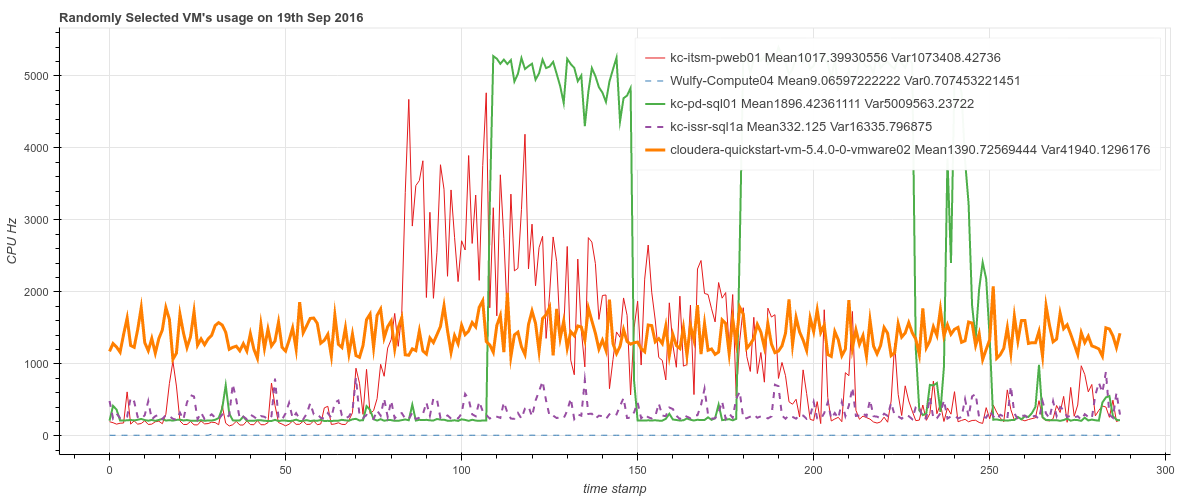
\includegraphics[scale=0.4]{sel_vms}
\centering
\caption{Randomly selected virtual machines, their mean and variance}
\label{fig:sel_vm}
\end{figure}

From Figure - \ref{fig:sel_vm}, it can seen that except virtual machine $Wulfy-Compute04$ all the other virtual machines have very high variance, which results in constantly varying values and predicting these virtual machine CPU utilization will be really difficult.

\subsection{Results}
\label{subsec:results}
Figures - ~\ref{fig:25_0_5} to \ref{fig:350} show the adaptive forecasted results of five randomly selected virtual machines for the day of $19^{th}$ Sep $2016$. It can be see that the negitive slope effect caused by methods with trend such as ES, ESWT, and linear regression are mitigated by using adaptive forecating technique with rectification. 

This method as it can be clearly seen from the figure -~\ref{fig:350} that the predicted signal tends to lag behind the actual value. This can be overcome by changing the step size or learning rate $l$ in equation - 11.

The effect of $l$ can be seen in figure -~\ref{fig:25_0_5} and~\ref{fig:25_1_0}. If there is a sudden variation in the cpu utilization, the prediction is larger than the actual value, which can be seen in figure -~\ref{fig:110}. However, if the same variation in the future occur, the prediction value is not as large as the previous value beacuse, the weights are adopted to reduce effect. WHich is not possible in simple forecating techniques such as exponential smoothing and exponential smoothing with trend.

As the forecasting is preformed through time, the weights are updated such that the more weight to given to the input which provide better prediction and less weights for the inputs with low importance in predicting the value. This phenomenon can be seen in figure -~\ref{fig:weights}. It can be seen form the figure that more weight is given to weighted moving avearge (WMA) followed by previous values (Prev) and lowest weight is given to exponential smooth with trend.

\begin{figure}[ht]
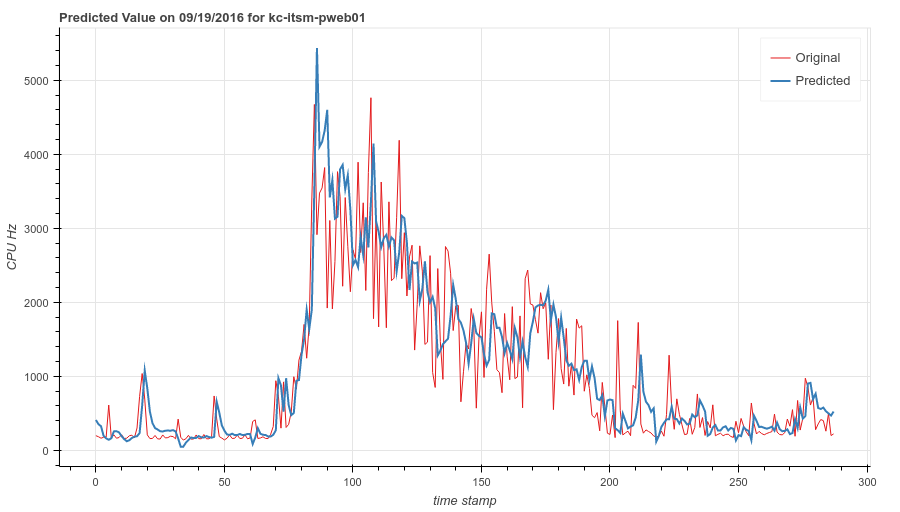
\includegraphics[scale=0.5]{2505}
\centering
\caption{Adaptive Forecating result on randomly seletced VM-1.}
\label{fig:25_0_5}
\end{figure}

\begin{figure}[ht]
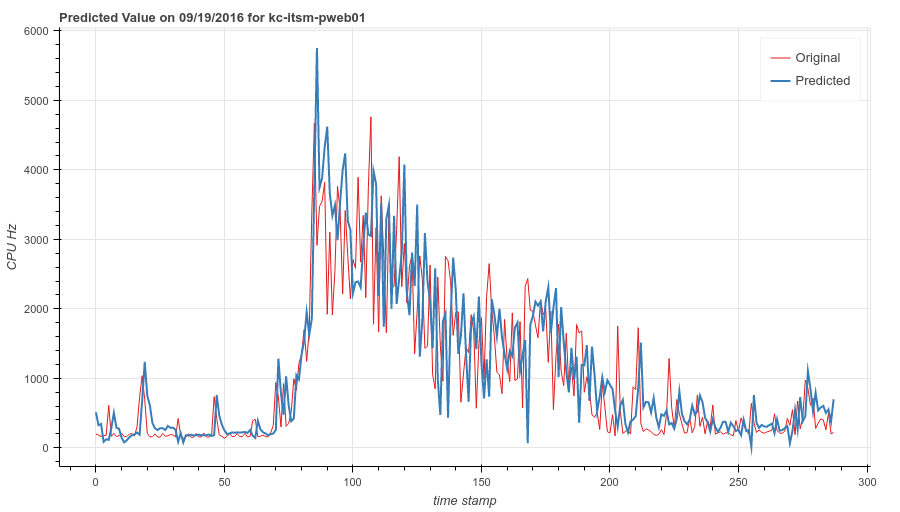
\includegraphics[scale=0.5]{2510}
\centering
\caption{Adaptive Forecating result on randomly seletced VM-1 with $l=1$.}
\label{fig:25_1_0}
\end{figure}

\begin{figure}[ht]
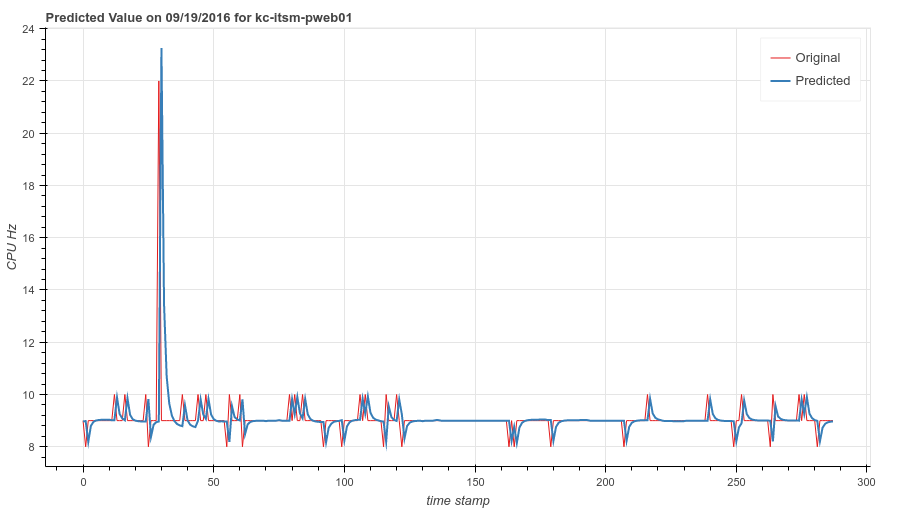
\includegraphics[scale=0.5]{60}
\centering
\caption{Adaptive Forecating result on randomly seletced VM-2.}
\label{fig:60}
\end{figure}

\begin{figure}[ht]
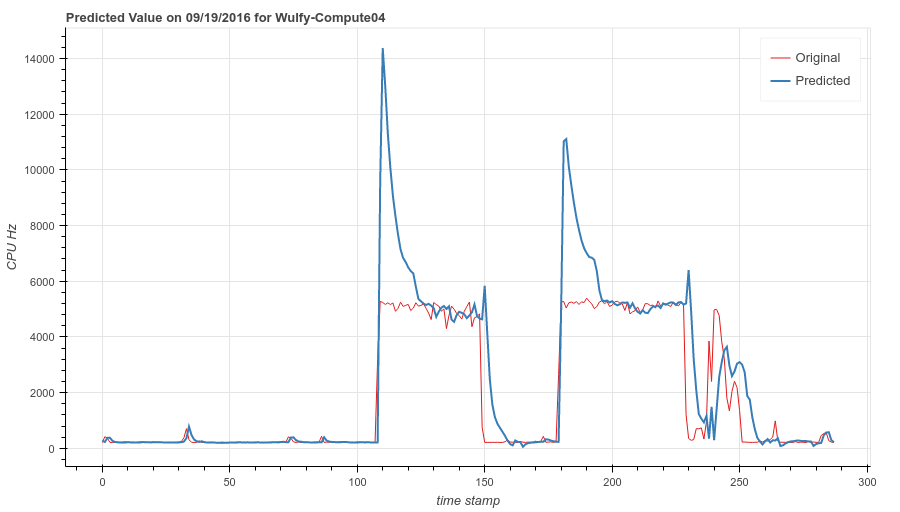
\includegraphics[scale=0.5]{110}
\centering
\caption{Adaptive Forecating result on randomly seletced VM-3.}
\label{fig:110}
\end{figure}

\begin{figure}[ht]
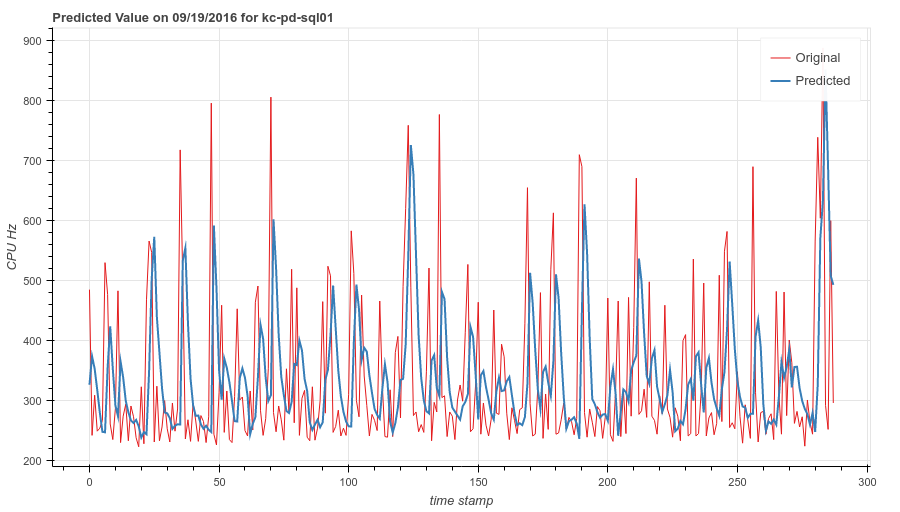
\includegraphics[scale=0.5]{225}
\centering
\caption{Adaptive Forecating result on randomly seletced VM-4.}
\label{fig:225}
\end{figure}

\begin{figure}[ht]
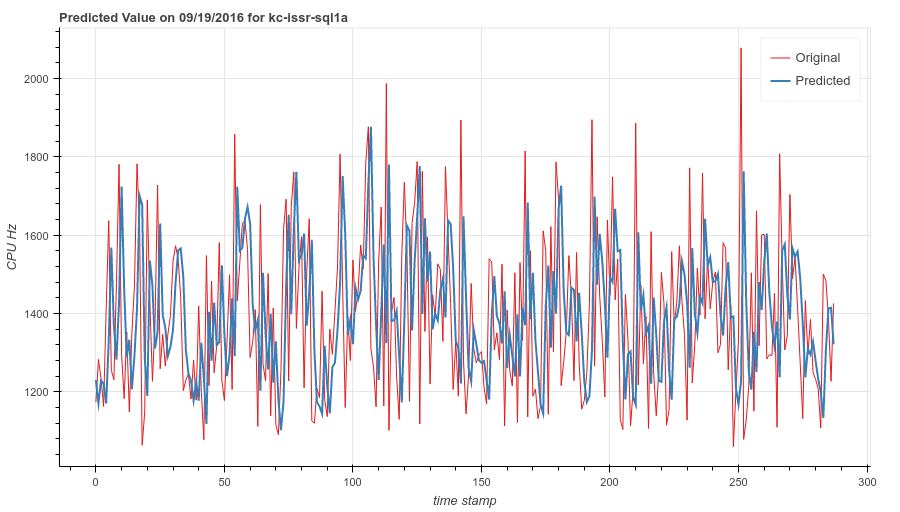
\includegraphics[scale=0.5]{350}
\centering
\caption{Adaptive Forecating result on randomly seletced VM-5.}
\label{fig:350}
\end{figure}

\begin{figure}[ht]
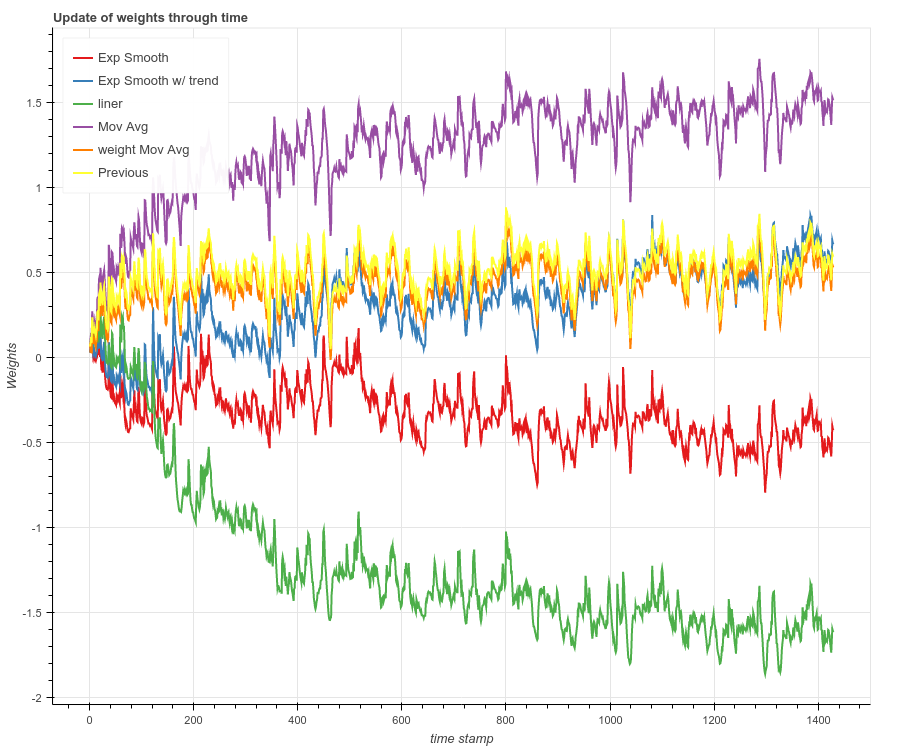
\includegraphics[scale=0.5]{weights}
\centering
\caption{The change in weights though time for VM-1.}
\label{fig:weights}
\end{figure}

\section{Conclusion}

In paper a neural networks based adaptive forecasting technique is used to predict the CPU utilization of virtual machines in UMKC datacenter. In this method multiple forecasting techniques such as moving average, weighted moving average, exponential smoothing and exponential smoothing with trend etc., will are used as input to the temporal neural network and these inputs are combine to predict the CPU utilization.  We also show how weights are updated for each input value through time.

In future, more tests will be conducted on this method and number of layers in neural network can be increased from single layer to multiple layers and also it is possible to increas number of input to the network by using differnet forecasting techniqes or atleast a window of previous values. The network in this paper is a simple linear unit. In future, nonlinearity can be added to this method to increase the performance of adaptive forecasting.

% Can use something like this to put references on a page
% by themselves when using endfloat and the captionsoff option.
\ifCLASSOPTIONcaptionsoff
  \newpage
\fi



\begin{thebibliography}{1}
\bibitem{ES} Fuqua School of Business {\em Moving average and exponential smoothing models} {\em http://people.duke.edu/~rnau/411avg.htm\#ses}.

\bibitem{ES2} NIST/SEMATECH {\em e-Handbook of Statistical Methods} {\em http://www.itl.nist.gov/div898/handbook/pmc/section4/pmc432.htm}

\bibitem{MWR} Wikipedia contributors {\em Regression analysis} {\em https://en.wikipedia.org/w/index.php?title=Regression\_analysis\&oldid=738229734}
\end{thebibliography}

\end{document}


